For the Petri net



\begin{centering}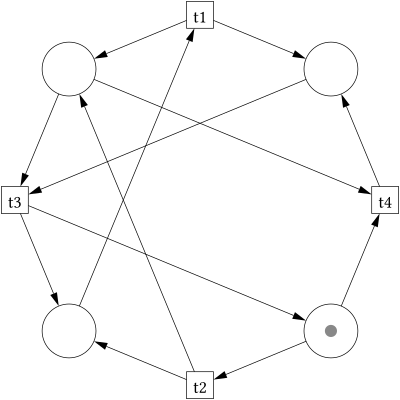
\includegraphics[min width=0.4\textwidth=0.6\textwidth,min height=0.4\textwidth=0.6\textwidth,keepaspectratio,max width=0.9\textwidth,max height=0.9\textwidth]{61/graph0petri0dbd941484c34cef8f33339c13cae5233c576107780d2064cb985289223481af01013.pdf}\end{centering}

a transition sequence is sought which leads to a marking without successors (i.e., to a deadlock).

State your solution as a sequence of the following kind that does not exceed 8 steps:


\begin{minted}{text}
[t1, t2, t3]
\end{minted}
Where giving these three steps means that after firing t1, then t2, and finally t3 (in exactly this order), the sought marking is reached.

Hint: There is no solution with less than 8 steps.

Please note: When hovering over or clicking on edges / nodes or their labels, the respective components that belong together are highlighted.